\lettrine[nindent=0em,lines=2]{T}he origins of superhydrophobicity research are traced to \cite{ollivier_1907}  where perfect sphere beads of water were observed on toxic arsenic trioxide and soot surfaces. Hydrophobicity arises on a surface from a lack of attractive forces causing water to 'repel' off the surface (\cite{Hydrophobicreview}).The self cleaning and superhydrophobic 'lotus effect' has fascinated researchers; research in the area has been re-energised by the discovery that \textbf{low surface energy} from epicuticle wax crystals as well as \textbf{surface roughness} from papillae are fundamental to the phenomena. The growth in interest is also spurred by its applications particularly in acid- rain building protection, self-cleaning surfaces and rust protection (\cite{LATTHE201952},\cite{SHSreview}). 
\par It is understood that low surface energy causes water droplets to bead up and potentially roll off. If the surface energy is high, water will spread out on the surface (e.g. glass) due to favourable interactions. The degree of hydrophobicity is characterised by the Water Contact Angle (WCA). An angle above 90$^\circ$ is hydrophobic and above 150$^\circ$ is superhydrophobic (\cite{SHSreview},\cite{ECOSHS}). 
\par To minimise surface energy, silanated compounds, particularly fluoroalkylsilanes, gain the most attention due to the greatest minimisation in surface energy. Despite being very effective, their high cost and toxicity to the environment has incentivised researchers to seek alternatives. Hence, it was discovered that the roughened metallic surface of CaCO$_3$ develops superhydrophobicity when functionalised with surfactants (\cite{demjen}). Fatty acids have been utilised due to commercial availability and reduced toxicity to the environment (\cite{SHENG20061983},\cite{HuDeng}, \cite{Cao}).The carboxylic acid head (hydrophilic)  chemisorbs onto the CaCO$_3$ surface seen in Figure \ref{calcium}, with the aliphatic tail orientated to provide surface hydrophobicity as well as physisorption from multiple layers of fatty acid (\cite{Kokkinis_2017}). 

\begin{figure}[h!]
\centering
  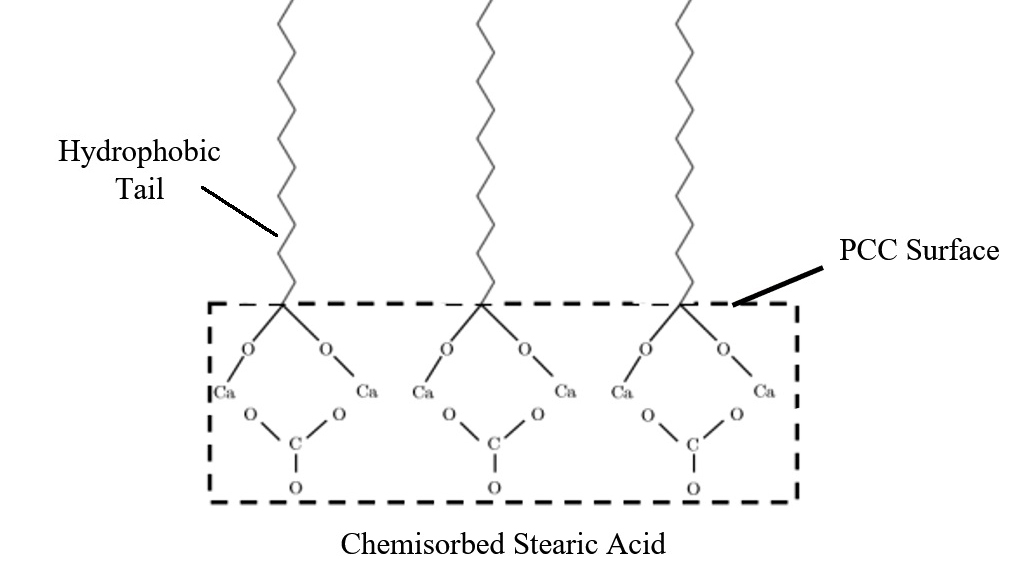
\includegraphics[width=0.35\textwidth]{Sections/Figures/SAFunctionalised4.jpg}
  \caption{Monolayer chemisorbed fatty acid functionalised CaCO$_3$ }\label{calcium}
\end{figure}

To form a monolayer, ball milling, pestle and mortar milling as well as wet methods such as a hot aqueous slurry have been used (\cite{Cao},\cite{DeArmritt}). Pestle and mortar dry milling was used in this project due to simplicity, no solvent and restricted access to laboratory equipment for ball milling. 

Stearic acid and Oleic acid, derived from sources such as cocoa butter and olives respectively, have been used as eco-surfactants and yielded successful SHP\footnote{Superhydrophobic Powder} using the mechano-chemistry technique rather than the wasteful solvent approach (\cite{deepika}). Stearic acid is one of the most suitable surfactants for calcium carbonate as it provides maximum surface coverage (\cite{gilbert_petiraksakul_mathieson_2001}). The powder was further optimised from hydrophobic to superhydrophobic with 2\%w/w stearic acid (\cite{Vatsal}.). Superhydrophobicity can also be attributed to the hierarchical structure of CaCO$_3$ that provides surface roughness as seen by SEM imaging (\cite{zhang_hierarchial}). The source of calcium carbonate has evolved from limestone and now can be derived from natural waste products such as eggshells (\cite{thailandshells}), and seashells (\cite{fang_2019}) enhancing sustainability.
\par Besides the superhydrophobicity of the powder,  there was an additional challenge of producing a sustainable paint (binder solution) so that a homogeneous coating can be practically applied. Due to environmental concerns, starch has received a lot of attention; as a natural biodegradable biopolymer, it is a promising candidate to replace the petroleum-derived materials currently in use. Starch already boasts a wide range of uses in industry - it is used in cosmetics, textiles, pharmaceuticals and fuels amongst others (\cite{kaur_ariffin_bhat_karim_2012}).  Amongst the candidates for petroleum replacement, starch is one of the most encouraging due to its diversity, film forming properties, availability, cost-effectiveness, and ease of handling (\cite{dufresne}, \cite{Caoprep}).  
\par Starch has been obtained from various botanical sources; as a consequence of its numerous sources, starch itself is a diverse polymer with different shapes, sizes, structures and chemical properties (\cite{smith_2001}). Starch contains two macro molecules: amylose (linear) and amylopectin (branched), with varying compositions allowing diverse physico-chemical properties of starch-based films. Corn Starch (Zea mays L.) was sourced with  28\% w/w amylose content  and a gelatinisation temperature of above 59.7 °C (\cite{luchese_spada_tessaro_2017}). Gelatinisation was essential to mitigate issues with cracking, hygroscopicity and non-continuous/inconsistent film formation (\cite{ZOBEL1984285}). Corn Starch was chosen as a starting point due to its low-cost and relatively high amylose content contributing to improved film flexibility, continuity and strength that occurs on cooling after gelatinisation (\cite{Amylosebenefit}).
\par Starch repeating units feature three free OH groups on each glycoside ring, making the molecule strongly hydrophilic. The OH groups make starch a promising binder due to H bonding with glass. Despite improving the binding ability, various starch hydrophobic functionalisation processes were reviewed to counteract the inherent hydrophilicity which reduces the hydrophobicity of the coating (\cite{wang}). \cite{jiang_dai_qin_xiong_sun_2016} demonstrated short-chain amylose starch modification in ethanol solution using 2-Octen-1-yl Succinic Anhydride (OSA) to produce amphiphilic OSA-starch-nanoparticles (OSA-SNP’s). The hydrophobicity of OSA-SNP’s increased with the degree of substitution as the OH groups on starch molecules were replaced by hydrophobic OSA groups. \cite{yu_jiang_zheng_cao_hou_xu_wang_jiang_pan_2019} formulated OSA-SNP powders which were pressed to obtain tablets; the starch modification had little effect on the particle size or morphology of starch, but increased the contact angle significantly, from 25.4° to 70.1°. The amphipathicity of modified starch polymers would increase the hydrophobicity of films over those that retained OH groups e.g.  unmodified corn starch. The OSA-Corn starch films were created using a modified method as described by \cite{OMSProcess}. 
\par The addition of inorganic tetraethylorthosilicate (TEOS) can also improve hydrophobicity of starch based-films (\cite{TEOS}) by the synergism of the components to form a starch-inorganic hybrid material. An adapted procedure was undertaken to prepare films by dip-coating with hydrolysis and condensation of TEOS in situ under a controlled pH, as demonstrated by \cite{TEOS}. 
\par Water molecules can also act as a plasticiser for hydrophilic polymers. \cite{wang_gu_hong_cheng_li_2011} demonstrated how the addition of silica nanoparticles at 10\% w/w corn starch not only increased shear strengths of starch-based binder but also increased the water resistance by 20.2\%, something invaluable for industrial applications in humid environments. Starch films incorporating silica nanoparticles were also investigated.

Producing superhydrophobic coatings that not only have a high WCA but are more sustainable is still a trending topic. (\cite{ECOSHS}). This year, water based PVA films have been produced (\cite{rewritable}) with 160° WCA as well as nano-CacO$_3$  films using Ethanol as a solvent but with 107° WCA. (\cite{syafiq_vengadaesvaran_ahmed_rahim_pandey_bushroa_ramesh_ramesh_2020}). There is limited research into using corn starch to develop superhydrophobic coatings. A recent superhydrophobic starch coating developed used expensive 80\% amylose corn starch , PDMS, Montmorillonite and a multi-step application process involving spraying/curing(\cite{chen_liu_yu_duan_ji_chen_2020}). Other superhydrophobic coatings developed utilise the developed SHP from CaCO$_3$ but use plastics such as Polyethylene and Polystyrene with a toluene solvent (\cite{Vatsal}).  Hence, there is a clear opportunity to combine the promising SHP with corn starch to produce superhydrophobic films. 

\subsection{Objectives}

This project aims to investigate the feasibility of replacing the  most recently optimised superhydrophobic coating using PE and Toluene (\cite{fang_2019}) with starch to produce a stable, homogenous film thus reducing harmful solvents and plastics in the environment. Various starch coatings will be produced in order to optimise the formulation. The efficacy of hydrophobic starches (see introduction) will be explored and quantified. The proposed coating must be able to be dried at ambient conditions and be applied simply by dip-coating.  The hydrophobic characteristics and durability of developed formulations will be compared and contrasted to the current formulation. 
\newpage
\subsection{Theory of Wetting Phenomena} 
Water contact angle (CA) is defined by the intersection of the three-phase boundary between solid, liquid and vapour. This is commonly described using Young’s equation:
\begin{equation}
\label{Young}
\gamma_s_v = \gamma_s_l + \gamma_l_v cos \theta_i
\end{equation}1
Here, $\gamma_s_v$, $\gamma_s_l$ and $\gamma_l_v$ denote the surface tensions of solid-vapour, solid liquid and liquid vapor respectively. $\theta_i$ denotes the ‘equilibrium’ CA on an \emph{ideal} surface i.e. one that is smooth, inert, homogeneous and nonporous. \cite{wenzel_1936} proposed an expression for the apparent equilibrium CA $\theta_w$ to account for surface roughness, as a function of roughness factor $r_f$
\begin{equation}
\label{Young}
cos \theta_w = r_f cos \theta_i
\end{equation}
This is valid when there is no gas trapped in between the droplet and crevices of the surface. When gas is trapped,  the Cassie and Baxter model is used: 
\begin{equation}
\label{Young}
cos \theta_c = \sigma (1+ cos \theta_i) -1
\end{equation}
Here the apparent CA ($\theta_c$) is a function of the relative fractional area of solid in contact with air, $\sigma$, and $\theta_i$ (\cite{cassie_baxter_1944}). In this model, the more air trapped between the liquid-solid interface, the higher the contact angle. 

However, static contact angle measurements alone aren’t sufficient to fully characterise a surface as using the average static CA neglects the irregularities of a real surface. One static, metastable CA only designates an angle within the range of contact angles possible between the advancing, $\theta_A$, and receding, $\theta_R$, contact angles; reporting the dynamic contact angles are therefore important criteria to further characterize the hydrophobicity of our film surfaces (\cite{gao_mccarthy_2006}). Hysteresis is the term used to describe this range between advancing and receding contact angles; it originates from and can indicate the properties that cause a surface to differ from the ideal, such as surface inhomogeneity and roughness. 

